\documentclass[pdf,bluish,slideColor,colorBG]{prosper}
\hypersetup{pdfpagemode=FullScreen}
\usepackage{color}
\usepackage{graphicx}
\usepackage{amsfonts}
\usepackage{amsmath}
\def\baselinestretch{0.7}
\parindent 0.3in
\hyphenpenalty=10000
\tolerance=10000
\pagestyle{empty}

\def\Prob{{\rm Prob\;}}
\def\prob{{\rm \;Prob\;}}
\def\Var{{\rm Var}}        % Var
\def\Cov{{\rm Cov}}        % Cov

\DeclareSymbolFont{AMSb}{U}{msb}{m}{n}
\DeclareMathSymbol{\expect}{\mathalpha}{AMSb}{'105}

% bold math (use \bm{...})
\def\bm#1{\mathpalette\bmstyle{#1}}
\def\bmstyle#1#2{\mbox{\boldmath$#1#2$}}

\title{Optimum selection and OU processes}

\author{Joe Felsenstein}

\institution{Biology 550D}

\subtitle{\small \\ 29 November 2016}


\definecolor{orange}{rgb}{1.0,0.8,0.0}
\definecolor{Dandelion}{rgb}{0.8,0.4,0.3}
\definecolor{golden}{rgb}{1.0,0.75,0.2}
%\definecolor{golden}{rgb}{1.0,0.8,0.3}
\definecolor{purple}{rgb}{0.6,0.2,0.6}
\definecolor{darkblue}{rgb}{0.1,0.1,0.6}
\definecolor{yellow}{rgb}{1.0,1.0,0.0}
\definecolor{brightred}{rgb}{1.0,0.,0.0}
\definecolor{black}{rgb}{0.0,0.0,0.0}
\definecolor{white}{rgb}{1.0,1.0,1.0}
\definecolor{purple}{rgb}{0.8,0.0,0.8}

% sets backgroundcolor for whole document 
%\pagecolor{darkblue}
%\pagecolor{white}
% sets text color
%\color{yellow}
%\color{black}
% to change just a few words
% using \textcolor{color}{text}

\DeclareSymbolFont{AMSb}{U}{msb}{m}{n}
\DeclareMathSymbol{\expect}{\mathalpha}{AMSb}{'105}

\def\Prob{{\rm Prob\;}}
\def\prob{{\rm \;Prob\;}}
\def\Var{{\rm Var}}        % Var
\def\Cov{{\rm Cov}}        % Cov

\begin{document}

% Source of covariation (VA, selective)
% 
% Ornstein-Uhlenbeck (Marguerite?)
% Chasing a peak
% Go where peak goes
% Smoothing caused by this
% Equilibrium covariances
% Tree covariation
% 


\maketitle

{
\parindent=0in

\begin{slide}[Replace]{With selection ... life is harder}

There is the ``Breeder's Equation'' of Wright and Fisher (1920's)
\[
\mathsf{\Delta z\ =\ h^2 S}
\]
\vspace{-0.10in}

\centerline{\includegraphics[width=1.0in]{Lande2011.ps}}
\medskip

and Russ Lande's (1976) recasting of that in terms of slopes of mean fitness
surfaces:
\vspace{-0.2in}

\[
\mathsf{S \ =\ V_P \; \frac{d \log\left({\bar w} \right)}{ d\bar{x}  }}
\]
\vspace{-0.2in}

\[
\mathsf{\Delta z\  =\  (V_A/V_P)\; V_P\; \frac{d \log\left({\bar w} \right)}{ d\bar{x} }
= \ V_A\;\frac{d \log\left({\bar w} \right)}{d\bar{x}  }}
\]

\noindent
Note -- it's heritability times the slope of log of {\it mean} fitness with
respect to {\it mean} phenotype.  There is an exact multivariate analog of
this equation.

\end{slide}

\begin{slide}[Replace]{Selection towards an optimum}
\bigskip

\centerline{\includegraphics[width=1.5in]{fig24-1.ydraw}}

If fitness as a function of phenotype is:
\[
\mathsf{w(x)\  = \ \exp\left[-\frac{(x-p)^2}{2 V_s } \right]}
\]
\vspace{-0.1in}

Then after some completing of squares and integrating,
the change of mean phenotype ``chases'' the optimum:
\[
\mathsf{m' - m\  =\  \frac{V_A}{V_s + V_P}\; (p - m)}
\]
\vspace{-0.1in}

\noindent
(There is an exact matrix analog of this for multiple characters).

\end{slide}

\begin{slide}[Replace]{The Ornstein-Uhlenbeck process}
\bigskip

(or rather, a random walk that comes interpolates it)

\[
\mathsf{x_{t+1} \ \ = \ \ x_t \ +  \ c\; (p - x_t) \ + \ \varepsilon_t}
\]

This is the same process as selection toward a peak value $~\mathsf{p}~$
plus genetic drift.  A process that wanders around an optimum but is
continually pulled toward it.
\medskip

It is easy to show (take expectations termwise) that the expectation of
$~\mathsf{x}~$ in the long run is $~\mathsf{p}$.

\end{slide}

\begin{slide}[Replace]{How variance accumulates in the OU process}
\bigskip

Subtracting $~\mathsf{p}~$ from both sides

\[
\mathsf{x_{t+1}\:-\:p \ \ = \ \ (1-c)(x_t\:-\:p)  \ + \ \varepsilon_t}
\]

Squaring both sides and taking expectations

\[
\mathsf{\expect[(x_{t+1}\:-\:p)^2] \ \ = \ \ (1-c)^2 \expect[(x_t\:-\:p)^2]  \
+ \ \expect[\varepsilon_t^2]}
\]

So that

\[
\mathsf{\Var(x_{t+1}) \ \ = \ \ (1-c)^2 \Var(x_t) \ + \ \Var(\varepsilon)}
\]

\end{slide}

\begin{slide}[Replace]{How variance accumulates in the OU process}
\bigskip

It is not too hard to show from this that

\[
\mathsf{\Var(x_t) \ \ = \ \ \Var(\varepsilon) \; \left(1 + (1-c)^2 + (1-c)^4 +
\dots (1-c)^{2t} \right)}
\]

Or in the limit
\[
\mathsf{\Var(x_\infty) \ \ = \ \ \frac{\Var(\varepsilon)}{1 \: - \: (1-c)^2}}
\]

If $~\mathsf{c}~$ is small, this is close to
\[
\mathsf{\Var(x_\infty) \ \ = \ \ \frac{\Var(\varepsilon)}{2c}}
\]
\bigskip

(Now we run the simulation of the OU process)

\end{slide}

\overlays{2}{
\begin{slide}[Replace] {Sources of evolutionary correlation among characters}
\bigskip

Variation (and covariation) in change of characters occurs for two reasons:

\begin{itemstep}
\item {\bf Genetic covariances}. (the same loci affect two or more traits)
\item {\bf Selective covariances} (Tedin, 1926; Stebbins 1950). The same
environmental conditions select changes in two or more traits -- even
though they may have no genetic covariance.
\end{itemstep}

\end{slide}
}

\begin{slide}[Replace]{A case that has received too little attention}
\bigskip

\begin{itemize}
\item Suppose characters $\mathsf{~x~}$ and $\mathsf{~y~}$ are genetically correlated.
\item and $\mathsf{~y~}$ is under optimum selection, but $\mathsf{~x~}$ is the one we observe.
\item What will we see?  In effect, the sum (actually, a weighted average) of
an Ornstein-Uhlenbeck process and Brownian Motion.
\item So Brownian motion restricted in the short run but not in the long run.
\end{itemize}

Most models so far do not allow for characters that are observed to covary with those that aren't observed.

\end{slide}

\begin{slide}[Replace]{Chasing a peak, simulated with two characters}
\bigskip

\centerline{\includegraphics[width=2.5in]{fig4.100.idraw}}

Genetic covariances assumed negative, but the wanderings of the adaptive peaks 
assumed positively correlated.
After a while (every generation up to generation 100), the wanderings of the peaks start to be
influential.

\end{slide}

\begin{slide}[Replace]{Chasing a peak, simulated with two characters}
\bigskip

\centerline{\includegraphics[width=2.5in]{fig4.1000.idraw}}

Genetic covariances assumed negative, but the wanderings of the adaptive peaks 
assumed positively correlated.
After a while (every 10th generation up to generation 1000), the wanderings of the peaks start to be
influential.

\end{slide}

\begin{slide}[Replace]{Chasing a peak, simulated with two characters}
\bigskip

\centerline{\includegraphics[width=2.5in]{fig4.10000.idraw}}

Genetic covariances assumed negative, but the wanderings of the adaptive peaks 
assumed positively correlated.
In the long run (every 100th generation up to generation 10,000) the means go mostly where the peaks go.

\end{slide}

\begin{slide}[Replace]{Other issues to think about}
\bigskip

\begin{itemize}
\item  What about multivariate drift and selection?
\item  What if the peak moves?
\item  What if the peak continues to move (and what is a natural assumption for
that process)?
\item  What happens at a speciation -- do both daughter species follow the
same adaptive peak, or different ones?
\end{itemize}

\end{slide}

\begin{slide}[Replace]{A little algebra showing the effect of selective covariance}
\bigskip

If we start from the familiar ``Breeder's Equation'' of quantitative genetics:
\[
\mathsf{\Delta z \ = \ h^2 \:S}
\]
it has long been known to have a multivariate version:
\[
\mathsf{\bm{\Delta z} \ = \ {\bf G} {\bf P}^{-1} {\bf S}}
\]

Multiplying $\bm{\Delta z}$ by its transpose:
\[
\mathsf{\bm{\Delta z} \bm{\Delta z}^T \ = \ {\bf G} {\bf P}^{-1} {\bf S} {\bf
S}^T {\bf P}^{-1} {\bf G}}
\]
and taking expectations (treating $\mathsf{\bf G}$ and $\mathsf{\bf P}$ as
constants) we get for the mean squares:
\[
\mathsf{\expect[\bm{\Delta z} \bm{\Delta z}^T] \ = \ {\bf G} {\bf P}^{-1} \expect[{\bf S} {\bf S}^T] \bf P^{-1} {\bf G}}
\]

\noindent
(Felsenstein, 1988)

\end{slide}

\begin{slide}[Replace]{References for multivariate Brownian motion}

Felsenstein, J.  2004.  {\it Inferring Phylogenies.}  Sinauer Associates,
Sunderland, Massachusetts. \textcolor{purple}{\bf [See particularly
chapters 23, 24, 25]}
\medskip

Felsenstein, J. 1988. Phylogenies and quantitative characters. {\it Annual
Review of Ecology and Systematics} {\bf 19:} 445-471. \textcolor{purple}{\bf [Review with mention of
usefulness of threshold model]}
\medskip

Felsenstein, J. 2002. Quantitative characters, phylogenies, and
morphometrics.pp. 27-44 in {\it Morphology, Shape, and Phylogenetics}, ed.
N. MacLeod. Systematics Association Special Volume Series 64. Taylor
and Francis, London.  \textcolor{purple}{\bf[Review repeating 1988 material and going into some
more detail on the question of threshold models.]}
\medskip

Lande, R. 1976. Natural selection and random genetic drift in phenotypic
evolution. {\it Evolution} {\bf 30:} 314-334. \textcolor{purple}{\bf [Lande's classic paper on drift versus
optimum selection]}
\medskip

Lande, R. 1979. The quantitative genetic analysis of multivariate
evolution, applied to brain-body size allometry. {\it Evolution} {\bf 33:} 402-416.
\medskip

\end{slide}

\begin{slide}[Replace]{References}

Lande, R. 1980. The genetic covariance between characters maintained
by pleiotropic mutations. {\it Genetics} {\bf 94:} 203-215.
\medskip

Lynch, M. and W. G. Hill. 1986. Phenotypic evolution by neutral mutation.
{\it Evolution} {\bf 40:} 915-935.
\medskip

Stebbins, G. L. 1950. {\it Variation and Evolution in Plants}. Columbia University
Press, New York. \textcolor{purple}{\bf [Describes selective covariance and cites Tedin (1925) for
it]}
\medskip

Tedin, 0. 1925. Vererbung, Variation, und Systematik der Gattung
{\it Camelina}. {\it Hereditas} {\bf 6:} 275-386.
\medskip

Armbruster, W. S. 1996. Causes of covariation of phenotypic traits among
populations. {\it Journal of Evolutionary Biology} {\bf 9:} 261-276. \textcolor{purple}{\bf [Good exposition of
selective covariance]}

\end{slide}
}

\end{document}


